% !TeX spellcheck = en_US
% !TeX root = ./0_article.tex

\section{Effects of BBI on IC operation}
\subsection{Extending the models: logic gates simulation}
	As we have stated previously, it is required, to complete the models, to properly consider the logical behavior of the considered circuits, which allows for a better appreciation of BBI induced effects and their consequences.
	These additional steps consist in modeling actual logic and sequential elements in the same or in a close technology as the considered IC, while extracting the significant disturbed signals from the SCS simulation and injecting them into these logic devices.
	For this purpose, we have divided this section into two subsections:
	\begin{itemize}
		\item A first section dedicated to studying a static logic gate: the classical inverter;
		\item A second section dedicated to studying an essential sequential element: the DFF.
	\end{itemize}

\subsection{BBI effects on static logic gates: inverters}
	% !TeX spellcheck = en_US
% !TeX root = ./0_article.tex

\begin{figure}[h]
	\label{ivxbufmos}
	\centering
	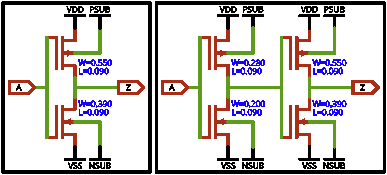
\includegraphics[width=0.5\textwidth]{./figures/IVX_BUFF_X4_3.pdf}
	\caption{IVX MOS SCH \textcolor{red}{A-T-ON LE DROIT DE METTRE CE SCHÉMA ?}}
\end{figure}

	Because inverters can have two stable output states, we will consider two cases for each substrate scenario: a normally high inverter (Fig. \ref{ivxbufmos}.a) and a normally low inverter (Fig. \ref{ivxbufmos}.b).
%		 as it is illustrated on the model shown in Fig. \ref{ivxbufmos}: a normally high and a normally low inverter.
	The inverters are connected to four external signals which are extracted from the previous SCS simulation:
	\begin{itemize}
			\item VDD: the power supply voltage;
			\item VSS: the power supply reference voltage;
			\item PSUB: the bulk voltage of the PMOS transistors;
			\item NSUB: the bulk voltage of the NMOS transistors.
		\end{itemize}
	The voltages PSUB and NSUB are different according to the substrate type.
	On the one hand, in the dual-well scenario, NSUB is connected to the epitaxial layer, while PSUB is connected to the N-well.
	On the other hand, in the triple-well scenario, NSUB is connected to the P-well and PSUB to the N-well.

	All of this gives us four scenarios to study.
	For clarity and because two of the four scenarios are less noteworthy, we will only talk about two of them:
	\begin{itemize}
		\item The triple-well substrate and the normally high inverter;
		\item The dual-well substrate and the normally low inverter.
	\end{itemize}
	Then, for each scenario, we will analyze seven signals of interest:
	\begin{itemize}
		\item The backside voltage pulse, for reference purposes;
		\item The local differential power supply voltage (VDD - VSS);
		\item The current sum of the inverter ($I_{DS}^{T1} + I_{DS}^{T2}$);
		\item The inverter load current, a.k.a. the current flowing through the capacitive output load;
		\item The inverter output voltage;
		\item The NSUB voltage (NMOS bulk voltage);
		\item the PSUB voltage (PMOS bulk voltage).
	\end{itemize}
	The signals extracted from the SCS simulations come from the standard-cell located directly below the BBI probe, a.k.a the cell targeted by the injection.
	% !TeX spellcheck = en_US
% !TeX root = ./0_article.tex

\begin{figure}[h]
	\centering
%	\vspace{\vsp mm}
	\subfloat[][Dual-well]{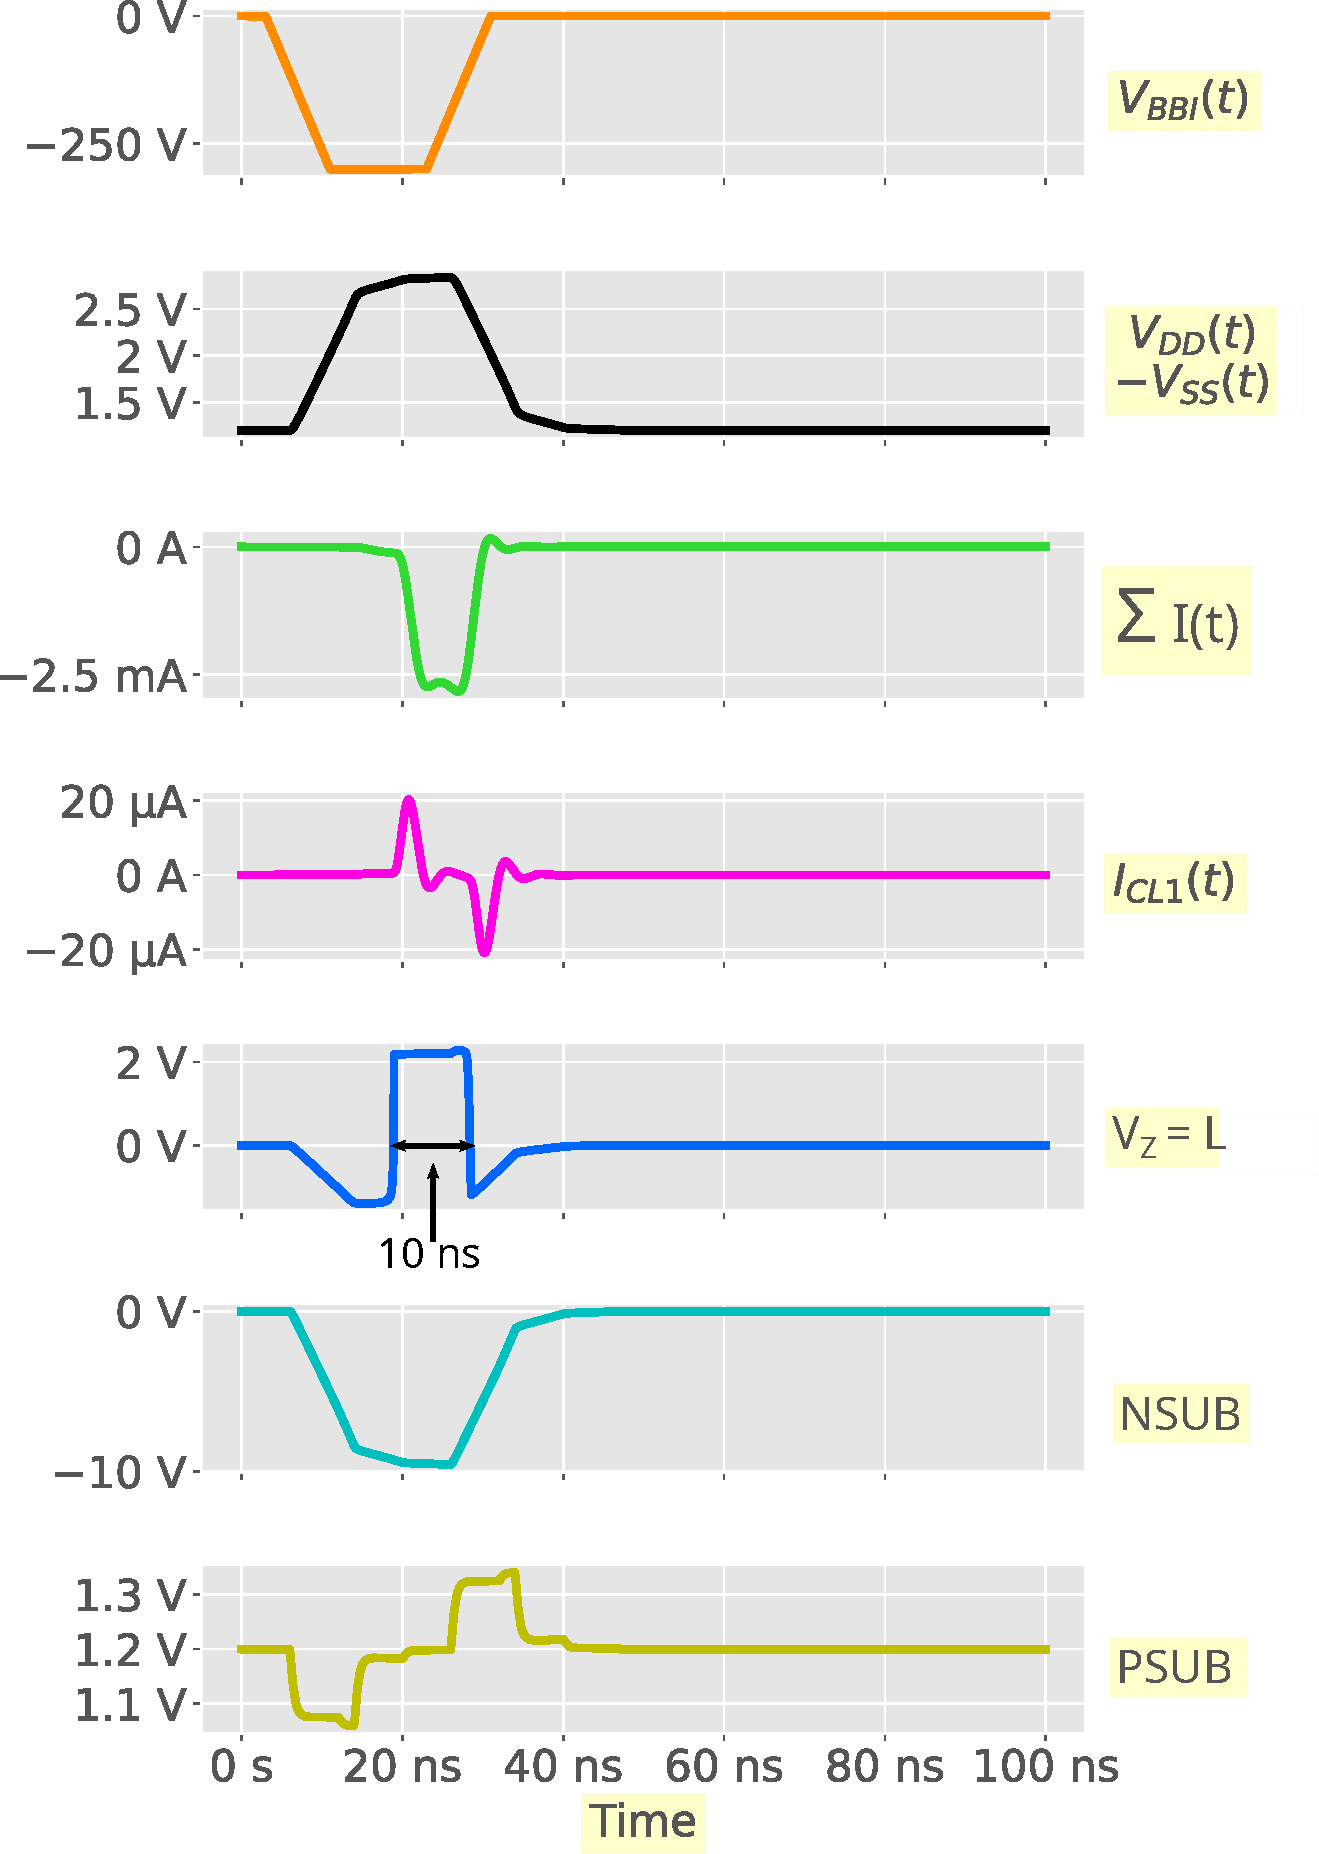
\includegraphics[width=0.506\columnwidth]{./figures/logic_gates_solo_M0_DW.pdf}}
	\subfloat[][Triple-well]{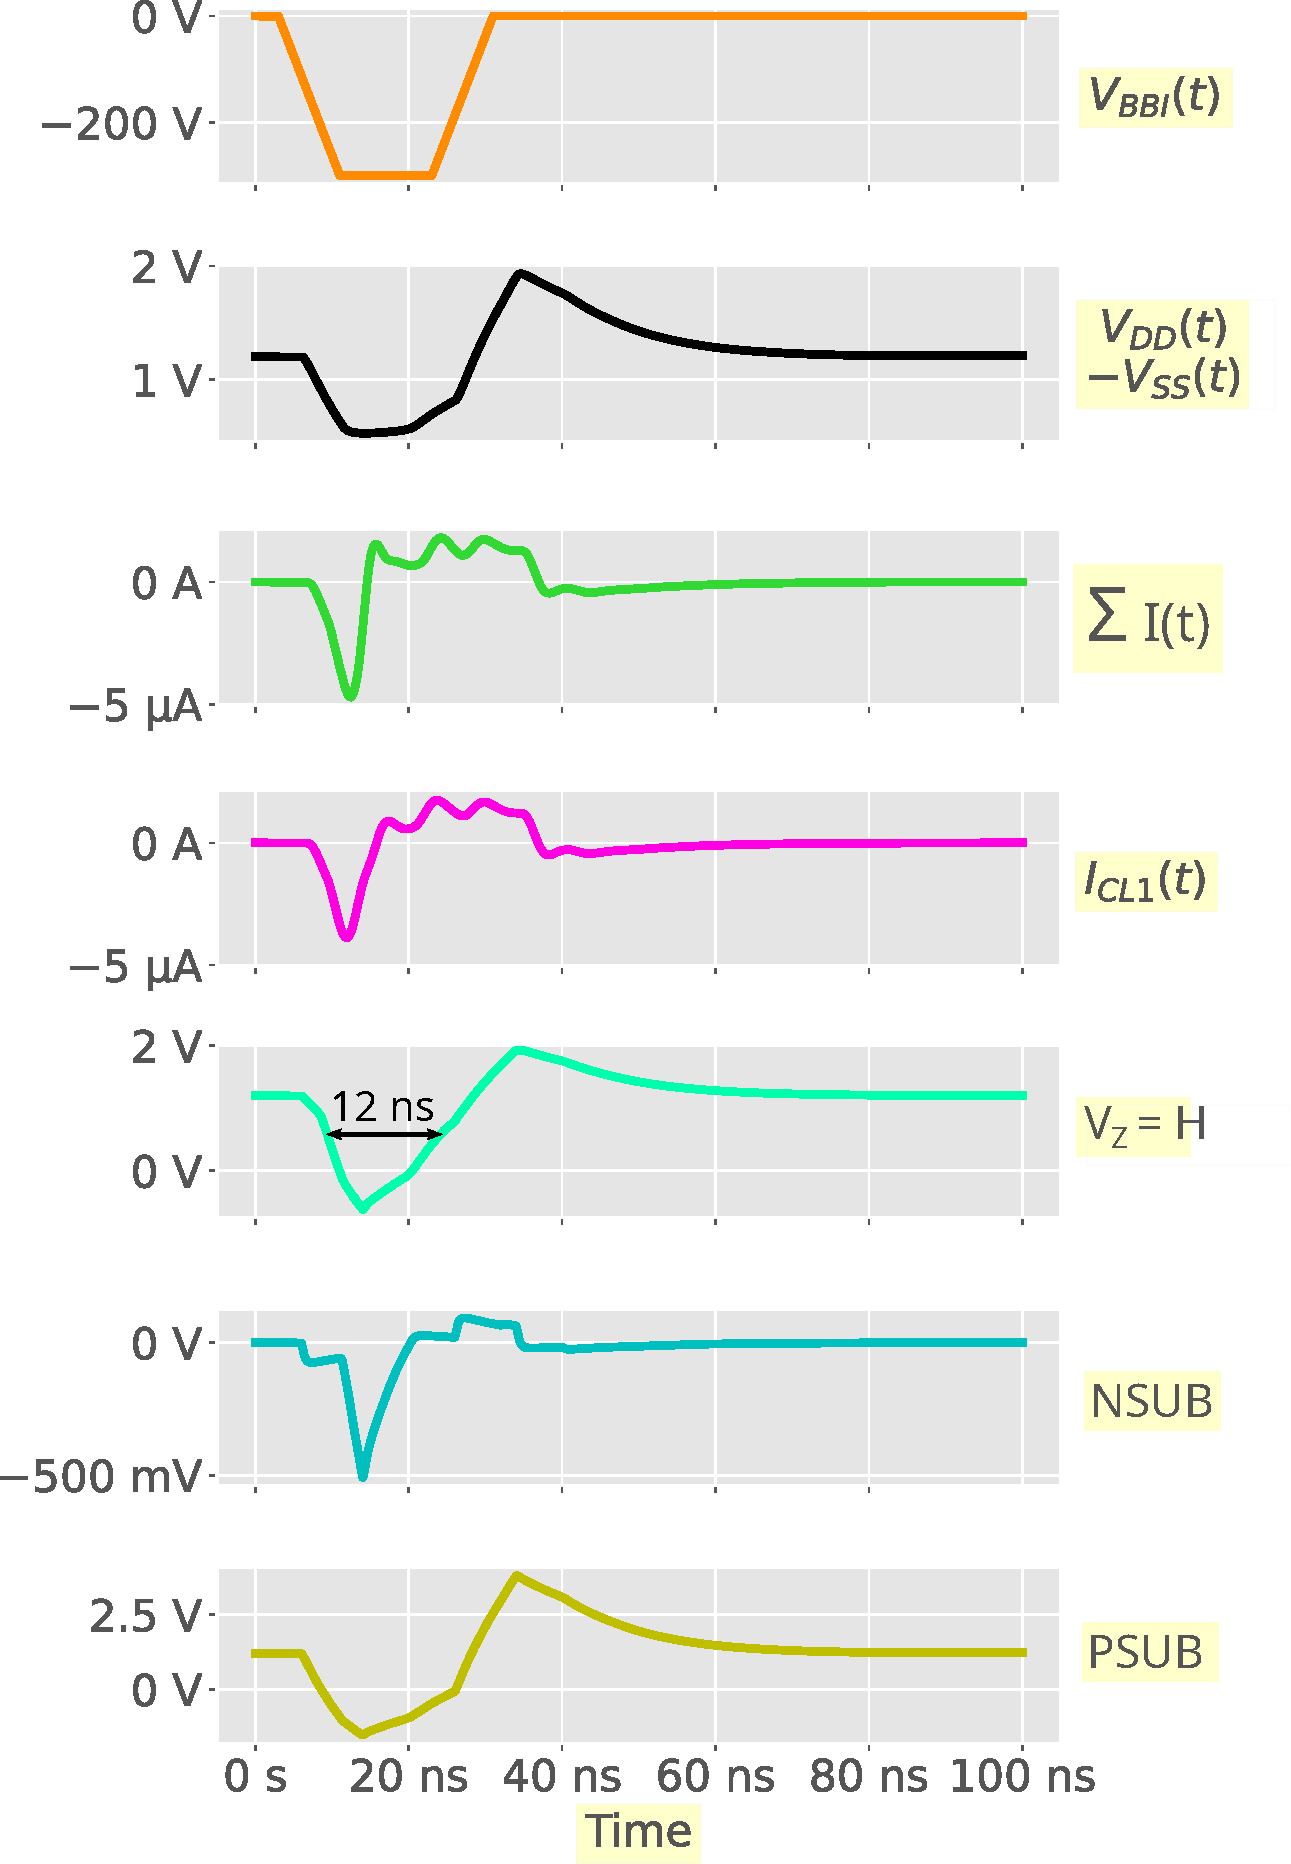
\includegraphics[width=0.494\columnwidth]{./figures/logic_gates_solo_M0_TW.pdf}}
	\caption{Inverters simulation results}
	\label{ivxsimu}
\end{figure}

	Fig. \ref{ivxsimu} presents the inverter simulation results for both considered scenarios.

	First, let us focus on the dual-well inverter.
	The corresponding schematic is shown in Fig. \ref{ivxbufmos}b, and the simulation results are shown in Fig. \ref{ivxsimu}a.
	In that case, as we have seen before, the global IC coupling is resistive, with a discrepancy between VSS and VDD: VSS being purely resistive, and VDD being purely capacitive.
	Therefore, the inverter current sum (green) follows a DC-response, similar to the differential power delivery voltage (black).
	The inverter output follows the current sum curve, and its output goes from a low to a high logic value during 10 ns, then back to its original state.
	It is further corroborated by looking at the load current, which is charged on the first pulse edge, then discharged on the second one.

	Second, concerning the triple-well inverter, where the results are shown in Fig. \ref{ivxsimu}b and the schematic in Fig. \ref{ivxbufmos}a, the substrate is globally AC-coupled.
	It can be seen on the current sum curve, which follows almost exactly the capacitive load current curve.
	The inverter output, for its part, is discharged like the load, and goes from a high logic value to a low value during 12 ns before returning to its original value.

	These observations are of great value because we can discuss a fault model for BBI, similar to what has been studied for EMFI and LFI.
	The previous results seem to indicate that the faults created using BBI are data-dependent.
	Indeed, if we lower the voltage of an inverter outputting a low value, or the opposite, it has theoretically no direct effect on the logic value.
	However, we have seen that it is possible, depending on the substrate type, to temporarily flip the value of a bit for the same amount of time than the pule width duration.
	Eventually, thanks to these results and the previous ones regarding current density in the substrate in Fig. \ref{sim_res_dw_neg}, \ref{sim_res_dw_pos}, \ref{sim_res_tw_neg} and \ref{sim_res_tw_pos}, it seems that BBI effects are local.

\subsection{BBI effects on dynamic logic gates: DFF}
	% !TeX spellcheck = en_US
% !TeX root = ./0_article.tex

\begin{figure}[h]
	\centering
	%	\vspace{\vsp mm}
	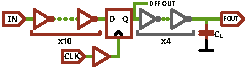
\includegraphics[width=\columnwidth]{./figures/dff_ivx_chain_3.pdf}
	\caption{DFF chain}
	\label{dffchain}
\end{figure}

	Now that we have analyzed the behavior of static inverters, it is important to consider studying the behavior of sequential elements such as a very common and widely used one: the D Flip-Flop.
%	These devices are used in every IC as an elementary memory element to sample data manipulated by the combinatorial logic.
	To test the DFF behavior under BBI, we placed it in the middle of a logic path and buffered its clock.
	The goal of this simulation is to mix the behavior of a disturbed logic path outputting to a disturbed DFF, itself outputting to a non-disturbed logic path.
	The non-disturbed path is here to mimic the behavior of far away logic gates receiving a disturbed signal while having a correct power supply.
	
	Similar to what we have done in the previous section, we will extract signals from the SCS simulation and inject them into the test circuit.
	The simplified schematic of such a circuit is shown in Fig. \ref{dffchain}.
	The first ten inverters, the buffer and the DFF are disturbed, while the last four inverters are not disturbed.
	The load $C_L$ mimics another set of logic gates which are loaded into the four inverters.
	As we did with the inverters, we will only consider negative pulses, both for a dual-well and a triple-well substrate.
	% !TeX spellcheck = en_US
% !TeX root = ./0_article.tex

\begin{figure}[h]
	\centering
	%	\vspace{\vsp mm}
	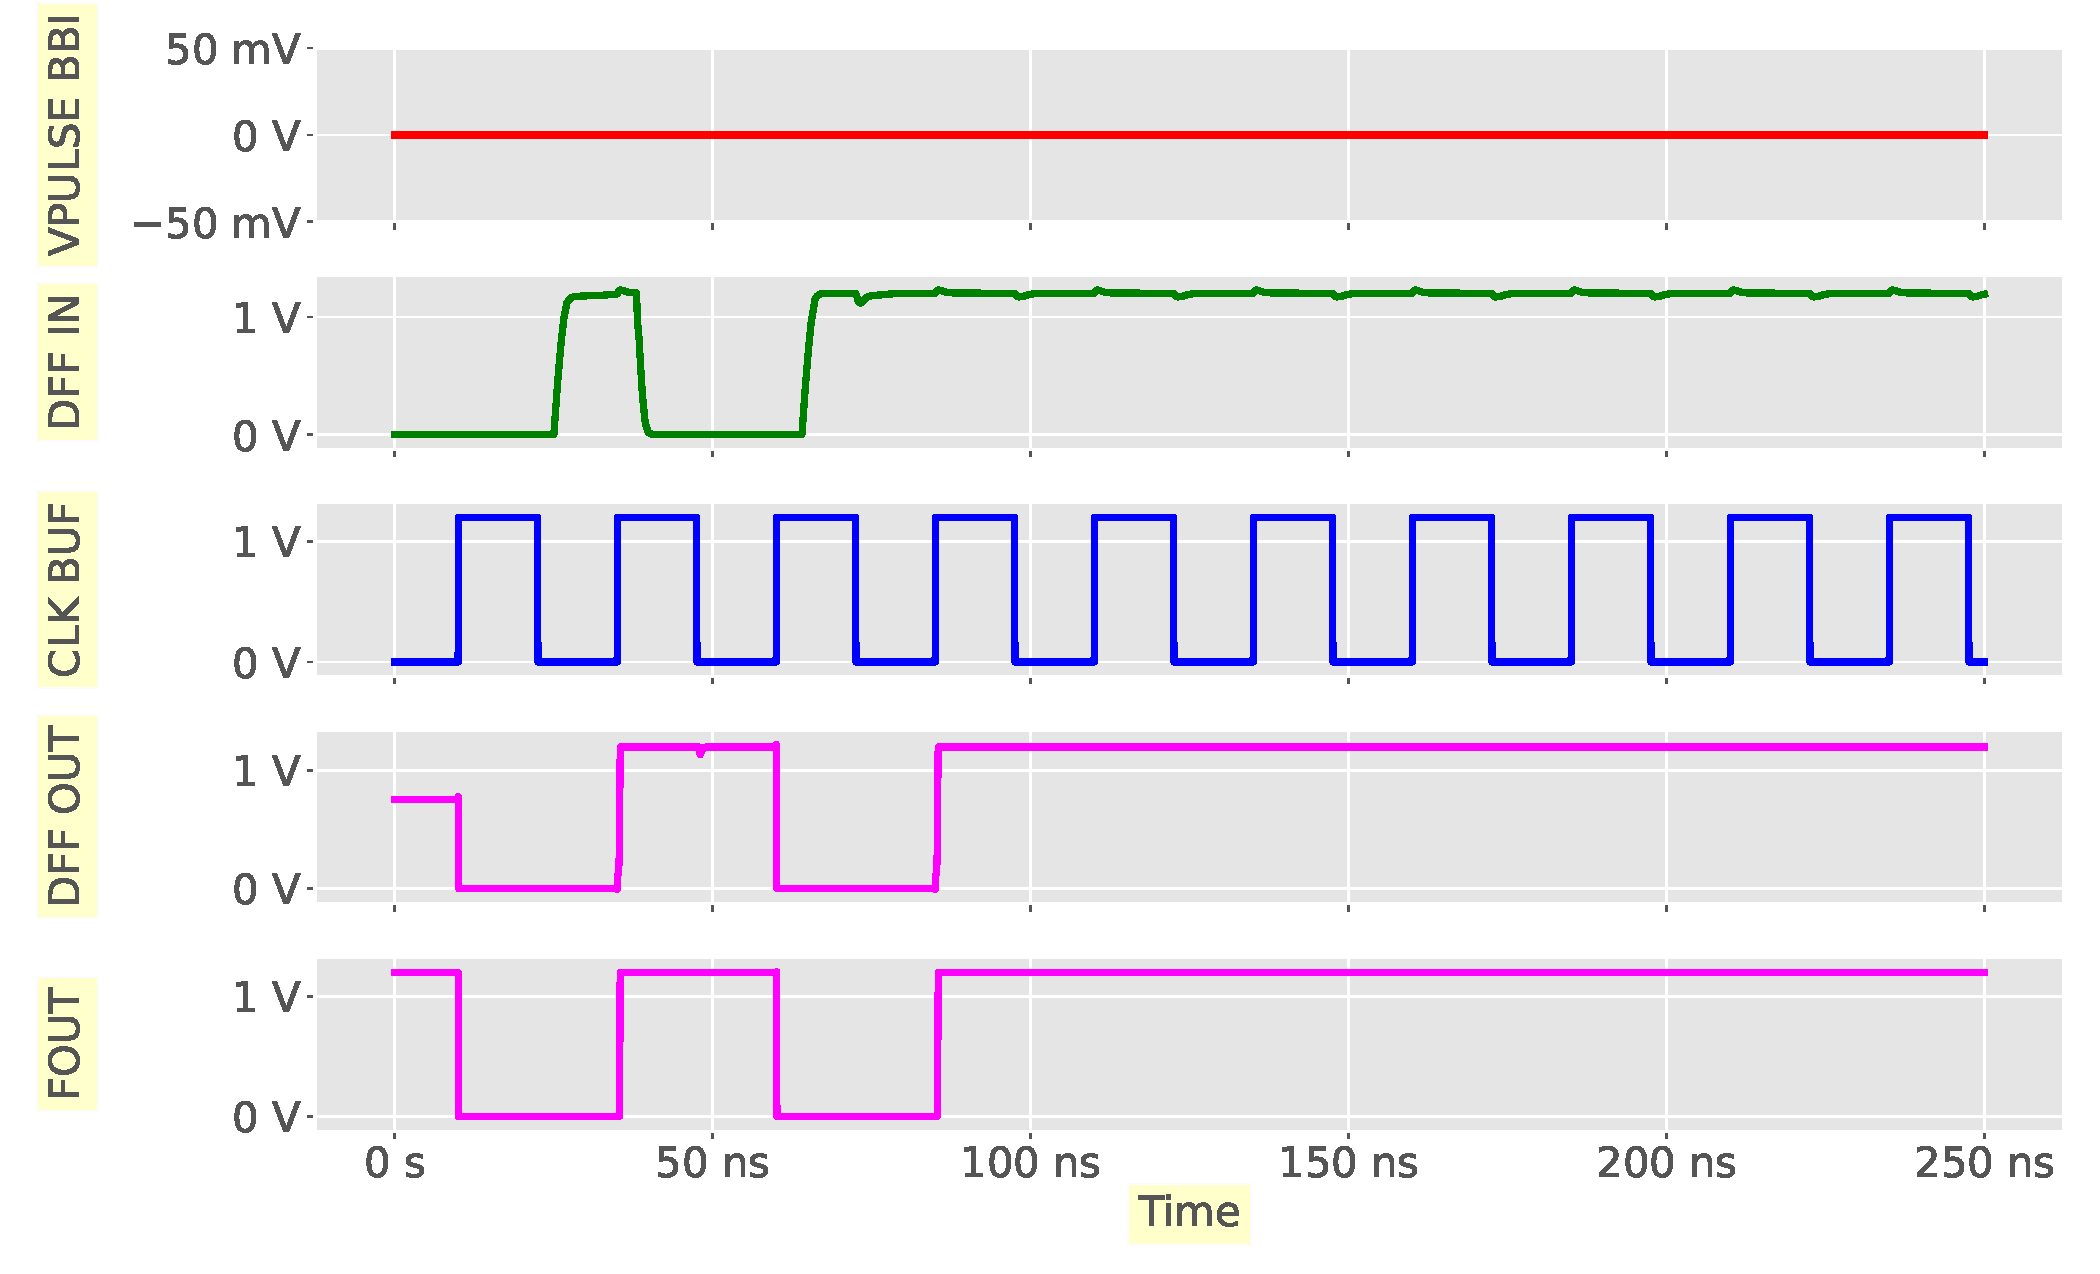
\includegraphics[width=\columnwidth]{./figures/anim0000-cropped.pdf}
	\caption{DFF path: idling}
	\label{dffidle}
\end{figure}

	Before diving into the simulation results, let us analyze what would be the normal behavior of the considered DFF.
	Fig. \ref{dffidle} presents the normal behavior of the modeled DFF path.
	The flip-flop is governed by a 40 MHz clock, similar to what we have used on our target, and we perform three data input sampling operations with alternating logic levels (High \textrightarrow\ Low \textrightarrow\ High), to finally let it rest at the last logic level.
	Because a DFF is a dynamic device, there are many interesting moments to observe depending on when the voltage pulse is injected.
	Therefore, we cannot represent every noteworthy moment, so we have chosen the most interesting ones.
	First, we will analyze the results where the injections are performed during the steady state of the DFF chain.
	Then, we will analyze the DFF behavior during the write operations.
%	During these simulations, we initialize the DFF with a low logic level, then a 
	
	\subsubsection{Dual-well substrate, negative pulse}
		% !TeX spellcheck = en_US
% !TeX root = ./0_article.tex

\begin{figure}[h]
	\centering
	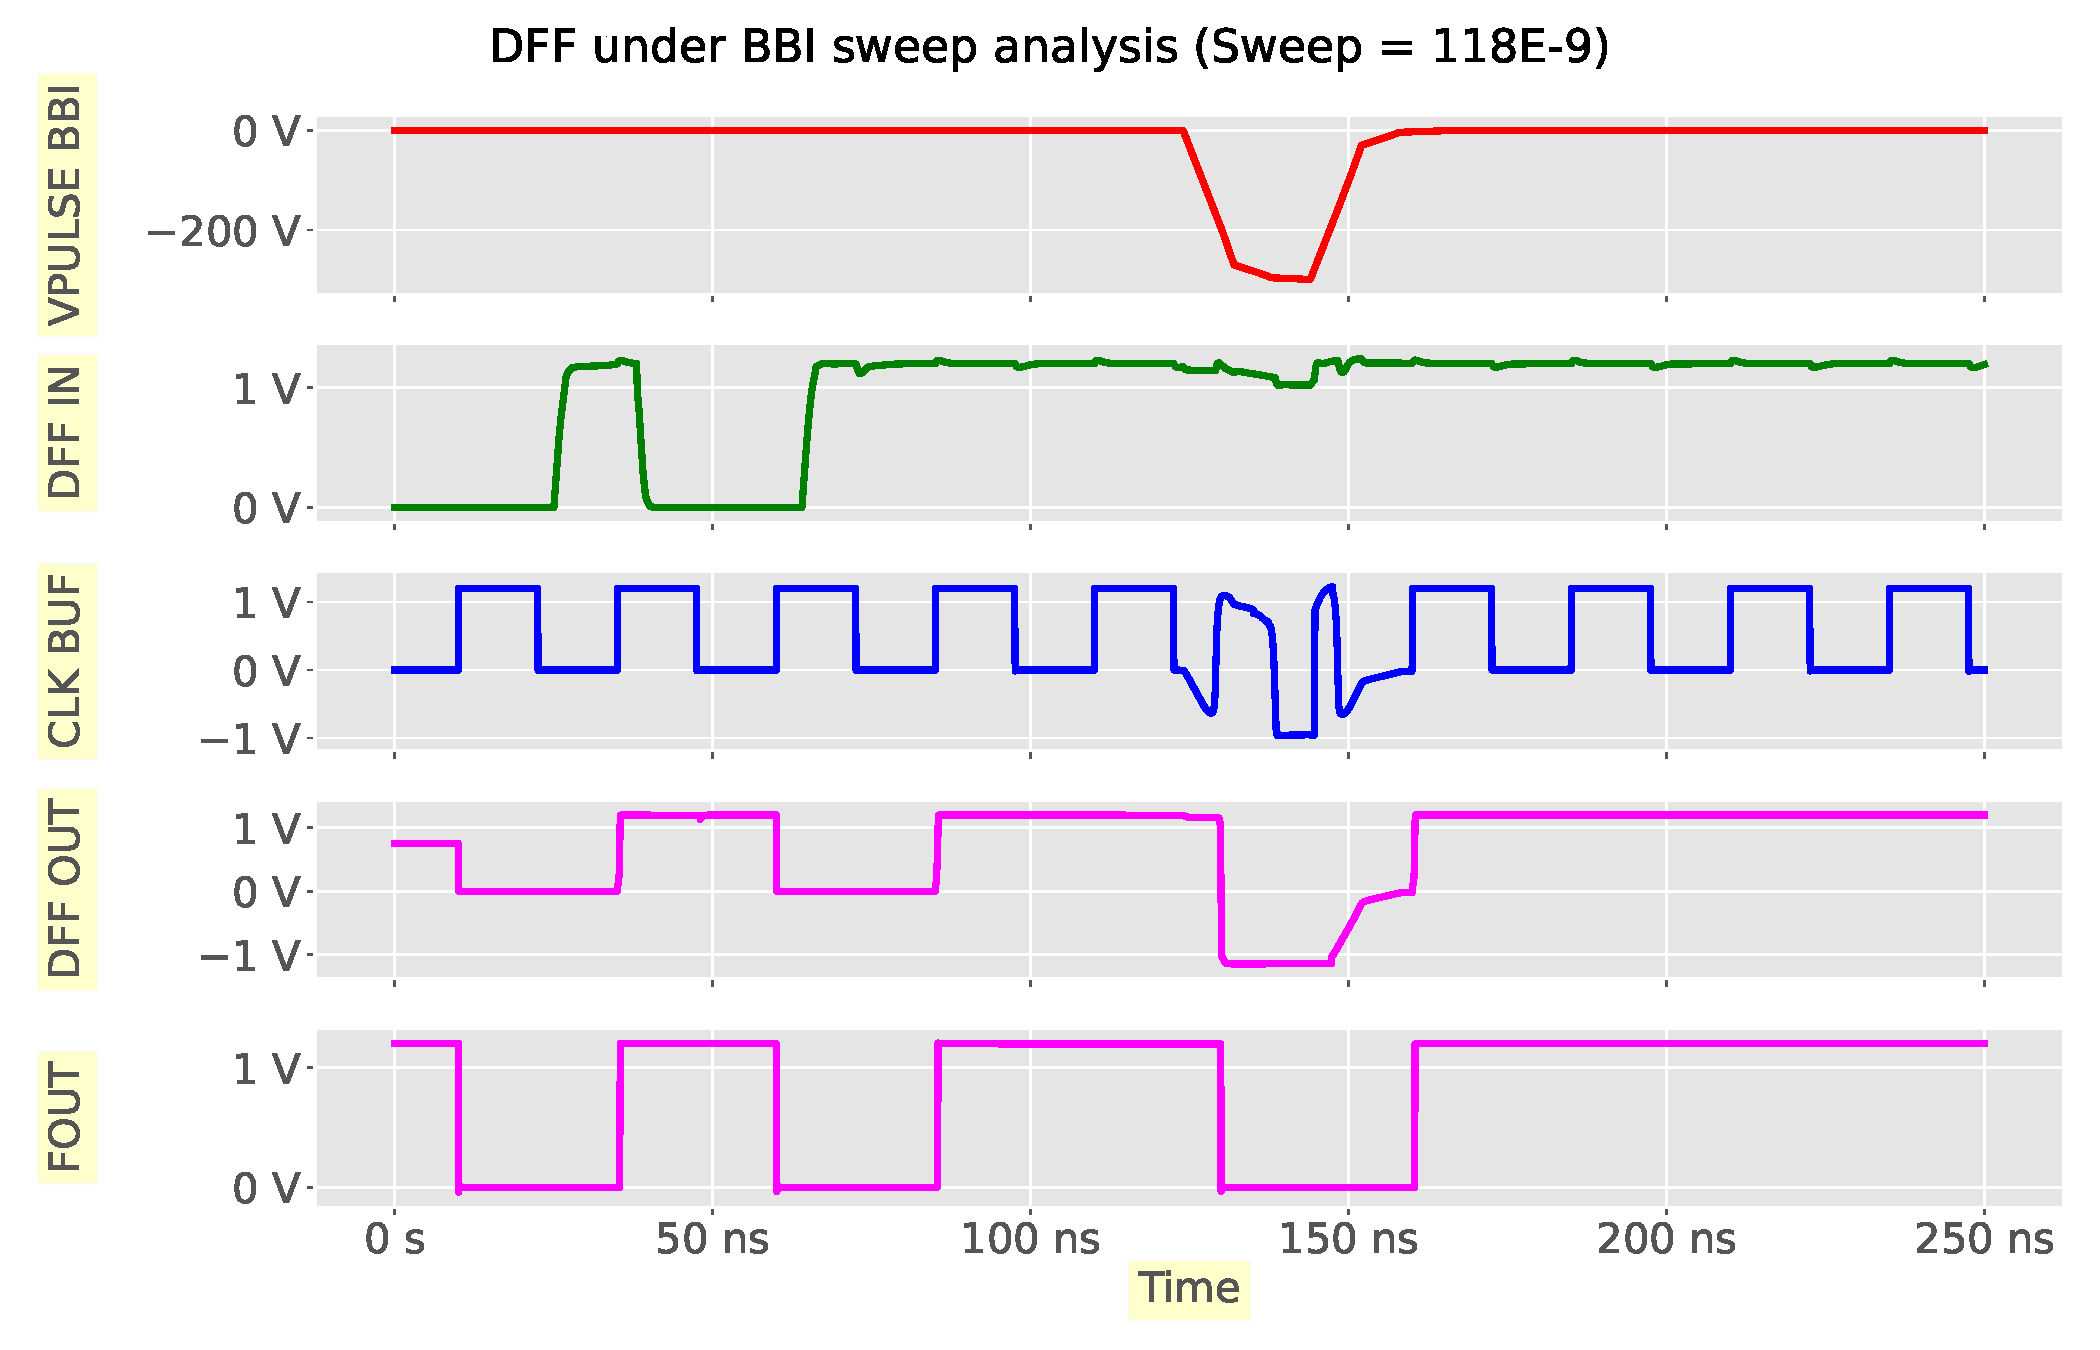
\includegraphics[width=\columnwidth]{./figures/dff-pdf-dw-neg/anim0108.pdf}
	\caption{DFF static DW}
	\label{dffstatic-dw}
\end{figure}

		Fig. \ref{dffstatic-dw} shows the simulation results for a dual-well negative pulse for a steady state disturbed DFF.
		Five signals are represented in this order, allowing us to get insights on the circuit behavior:
		\begin{itemize}
			\item The BBI voltage pulse for reference;
			\item The DFF input signal (DFF IN), being the output of the first ten inverters;
			\item The buffered DFF clock (CLK BUF), the clock fed to the DFF after the buffer;
			\item The DFF output;
			\item The four last inverters output;
		\end{itemize}
		The results show that the DFF input is not disturbed enough to trigger a logic value change.
		However, the DFF output drops down to -1 V, similar to its own buffered clock.
		This voltage drop, lasting for 25 ns, reverberates on the clean inverters output, resulting in a low logical value being output.
		In addition to this, the disturbances on the clock shows the creation of two parasitic clock pulses, replacing a normal one during the injection.
		
		% !TeX spellcheck = en_US
% !TeX root = ./0_article.tex

\begin{figure}[h]
	\centering
	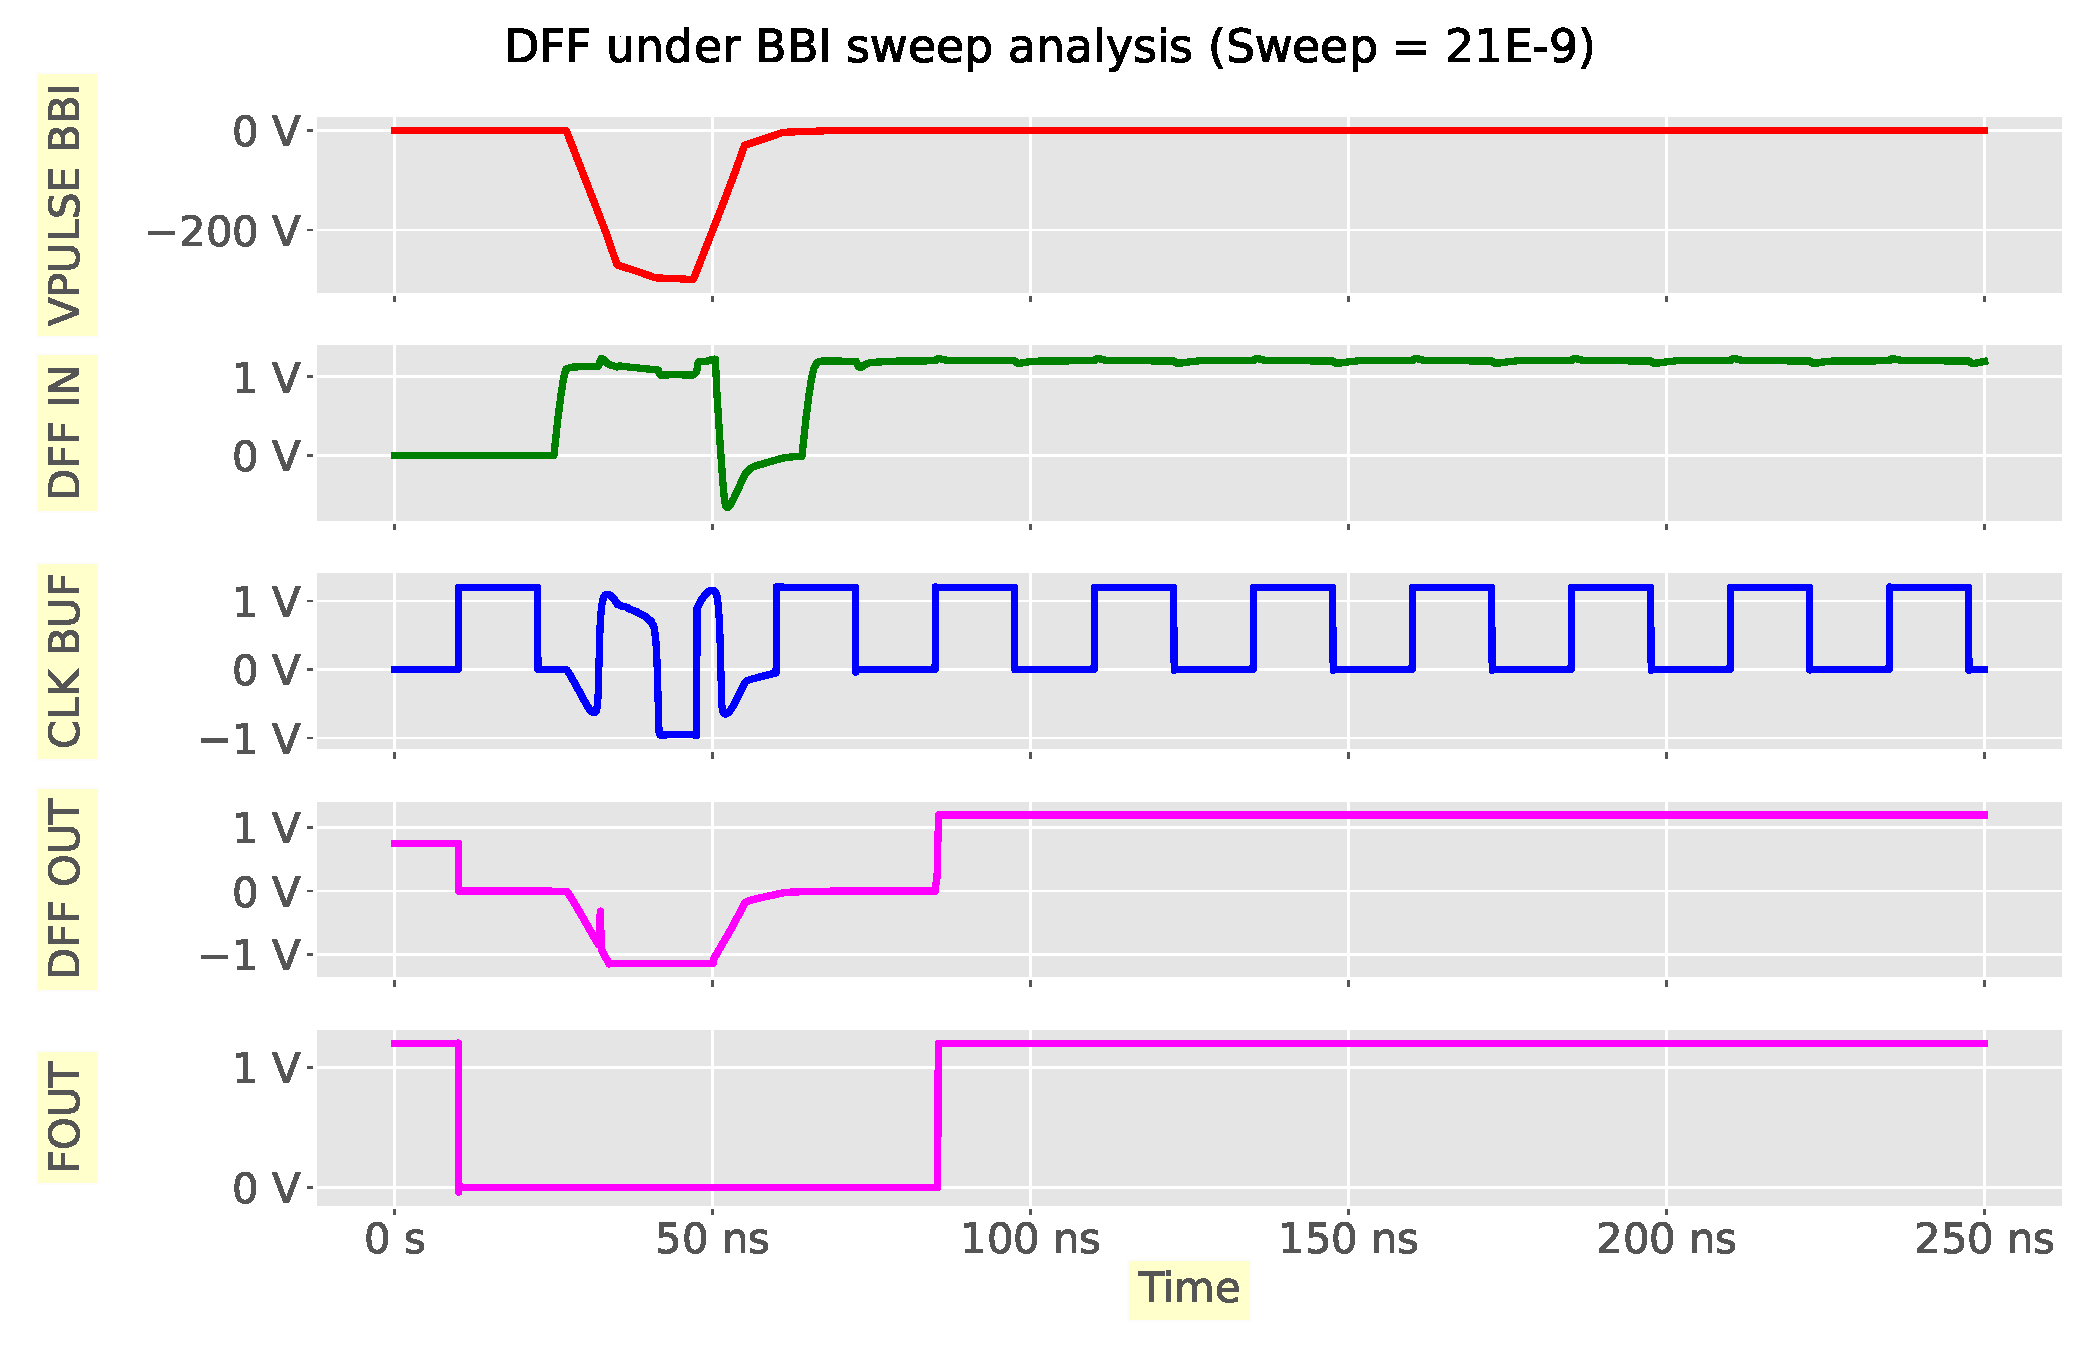
\includegraphics[width=\columnwidth]{./figures/dff-pdf-dw-neg/anim0011.pdf}
	\caption{DFF path: dynamic dual-well}
	\label{dffdynamic-dw}
\end{figure}

		Then, Fig. \ref{dffdynamic-dw} shows the exact same scenario with a different injection time, performed during the first write operations.
		These results show that the disturbances prevent the second write operation, supposed to write a high logic value in the DFF.
		Therefore, this data will never be sampled by the DFF and therefore will never propagate to the output of the circuit.
	
	\subsubsection{Triple-well substrate, negative pulse}
		% !TeX spellcheck = en_US
% !TeX root = ./0_article.tex

\begin{figure}[h]
	\centering
	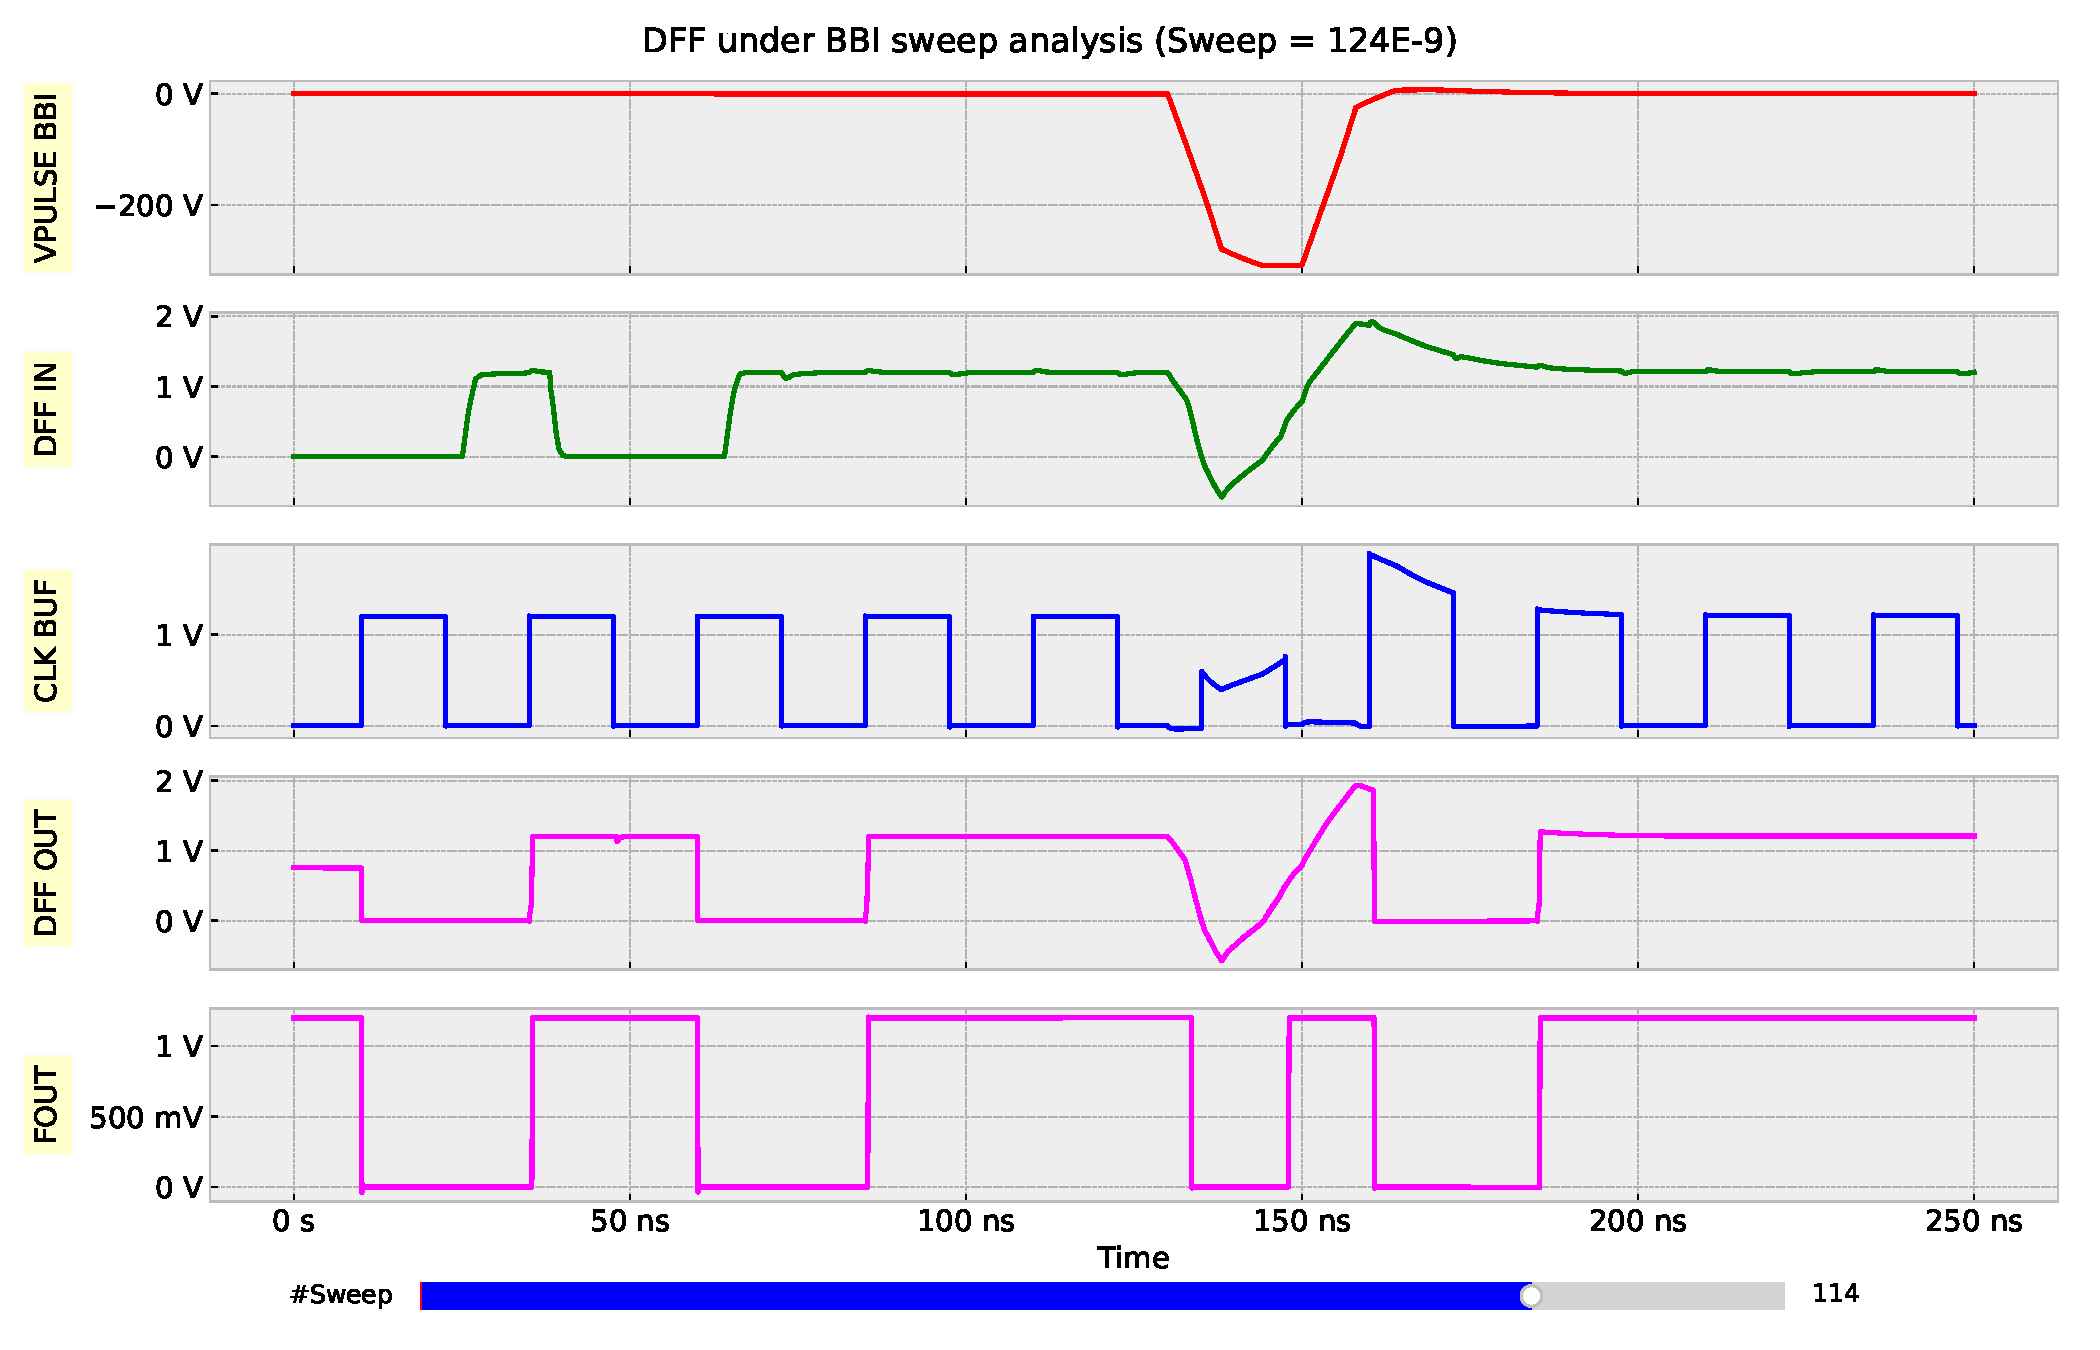
\includegraphics[width=\columnwidth]{./figures/dff-pdf-tw-neg/anim0114.pdf}
	\caption{DFF path: static triple-well}
	\label{dffstatic-tw}
\end{figure}

		Fig. \ref{dffstatic-tw} shows the simulation results for a triple-well negative pulse for a steady state disturbed DFF.
		In that case, the DFF input is disturbed, similarly to its output, by the BBI pulse.
		This causes a voltage drop significant enough to create a parasitic low logical value at the net FOUT.
		Concerning the clock, its maximum voltage is damped by the BBI pulse down 700 mV for one period.
		
		% !TeX spellcheck = en_US
% !TeX root = ./0_article.tex

\begin{figure}[h]
	\centering
	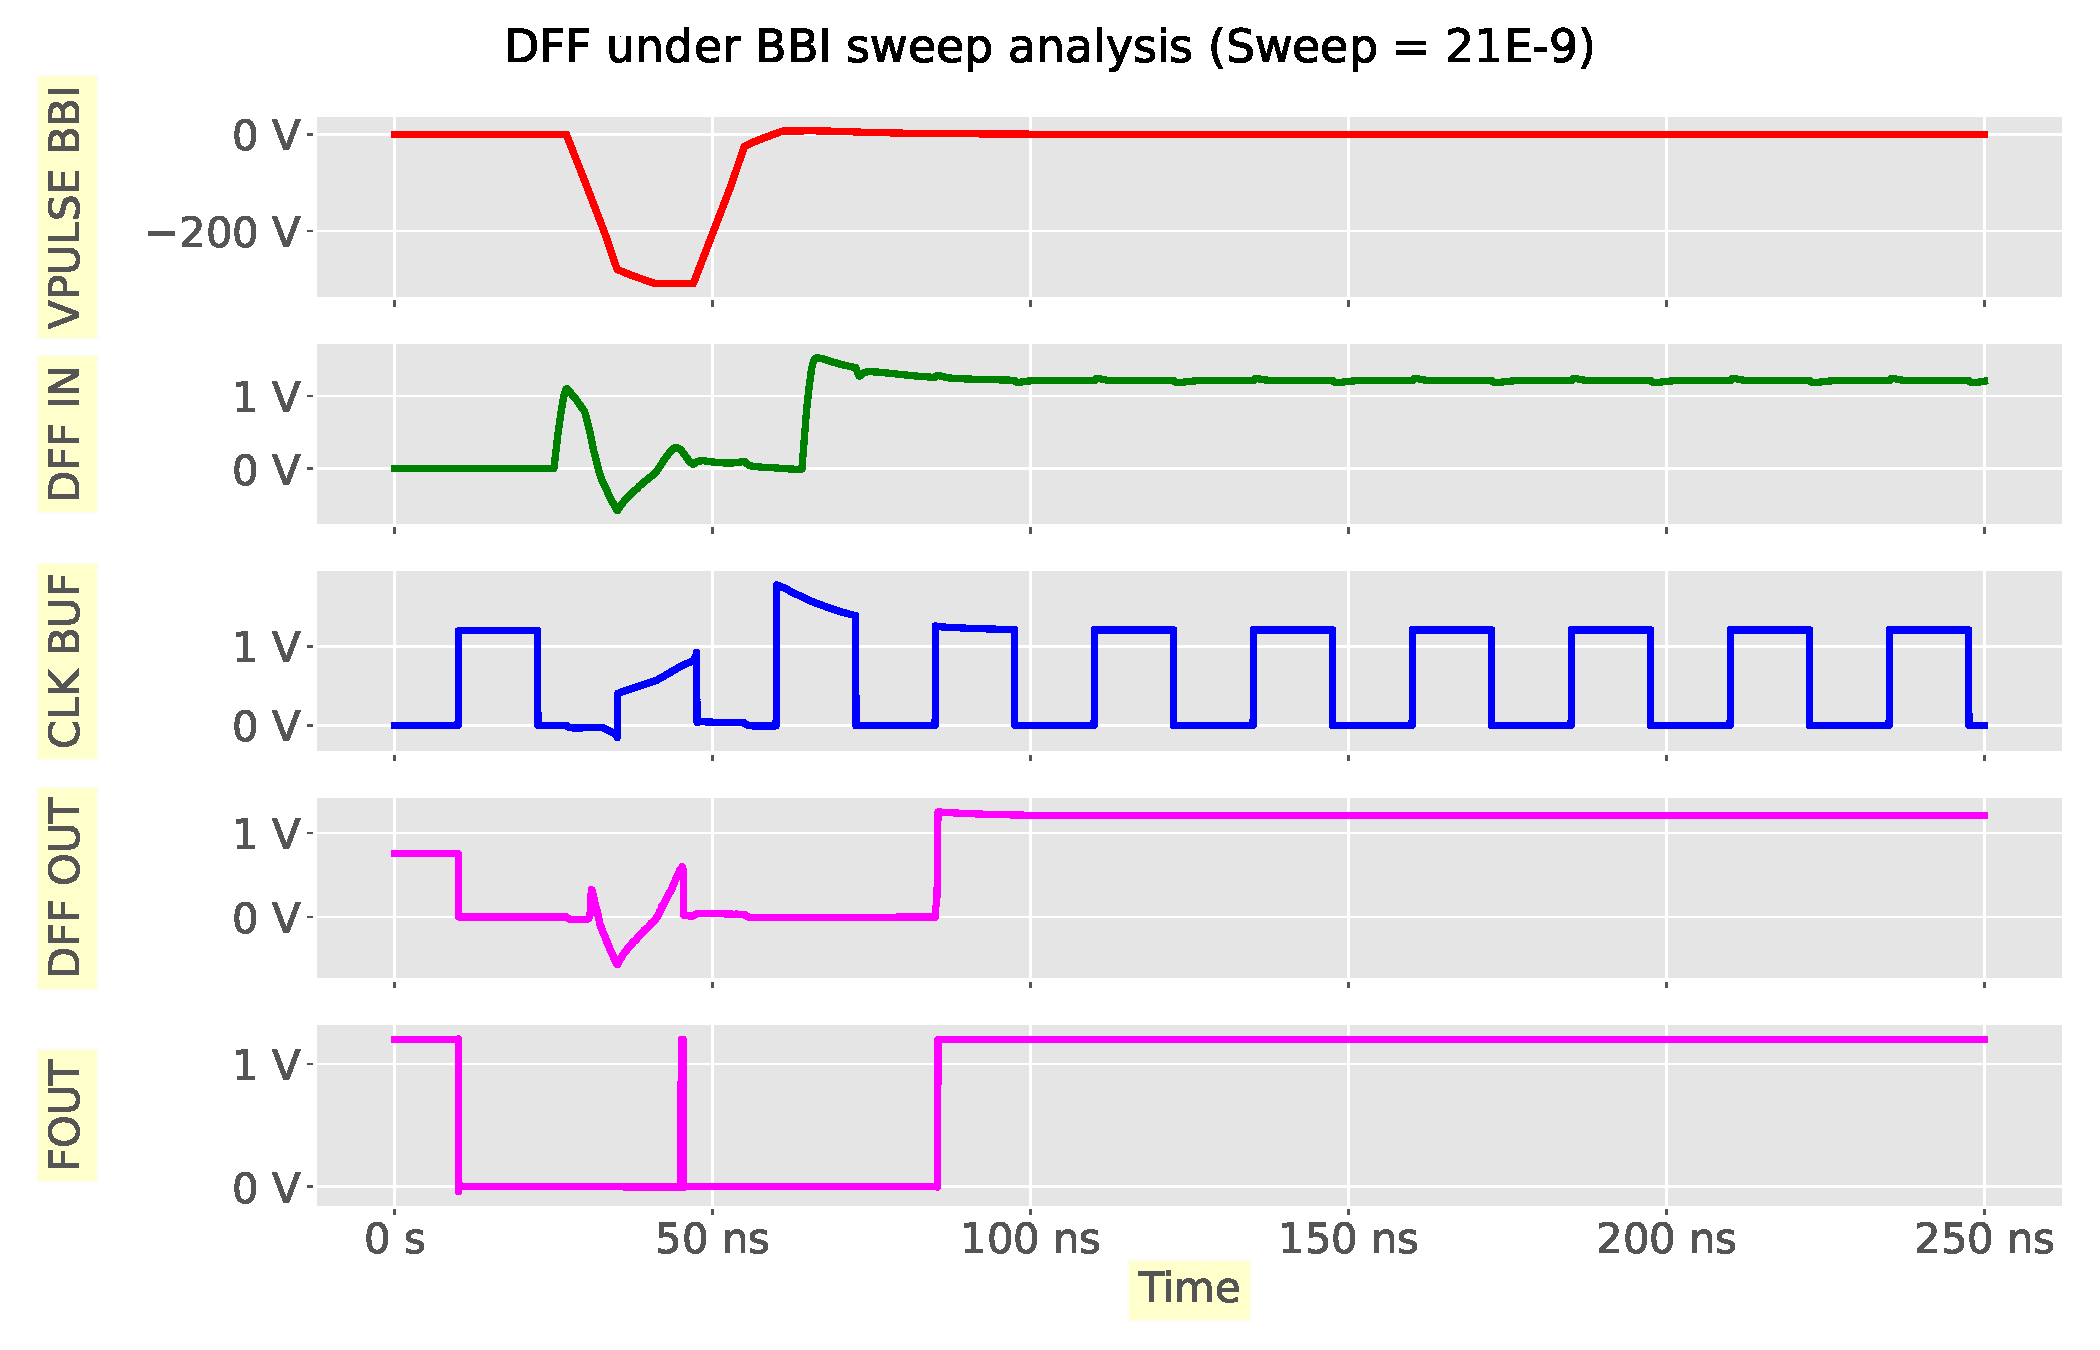
\includegraphics[width=\columnwidth]{./figures/dff-pdf-tw-neg/anim0011.pdf}
	\caption{DFF path: dynamic triple-well}
	\label{dffdynamic-tw}
\end{figure}

		Eventually, Fig. \ref{dffdynamic-tw} shows the results for a dynamic BBI in a triple-well under a negative pulse.
		Similar to the steady state result, the clock voltage is damped down to 800 mV.
		The DFF input is clearly disturbed and the disturbance follows the BBI pulse, which is similar on the DFF output.
		These disturbances then cause an error during the sampling of the high logic value, which reverberates on the net FOUT, which shows a short pulse instead of a plateau, around 50 ns.
		
\subsection{BBI effects on dynamic logic gates: DFF in practice}
	\textcolor{orange}{The rest of this section is in the making. Some experiments are missing to illustrate the DFF results. We are waiting for the newly opened circuits.}

%	For this purpose, we modeled an inverter, a buffer and a DFF.
%	The inverter and the buffer schematics, alongside their transistors sizes, are shown in Fig. \ref{ivxbufmos}.
%%	% !TeX spellcheck = en_US
% !TeX root = ./0_article.tex

\begin{figure}[h]
	\label{dffmos}
	\center
	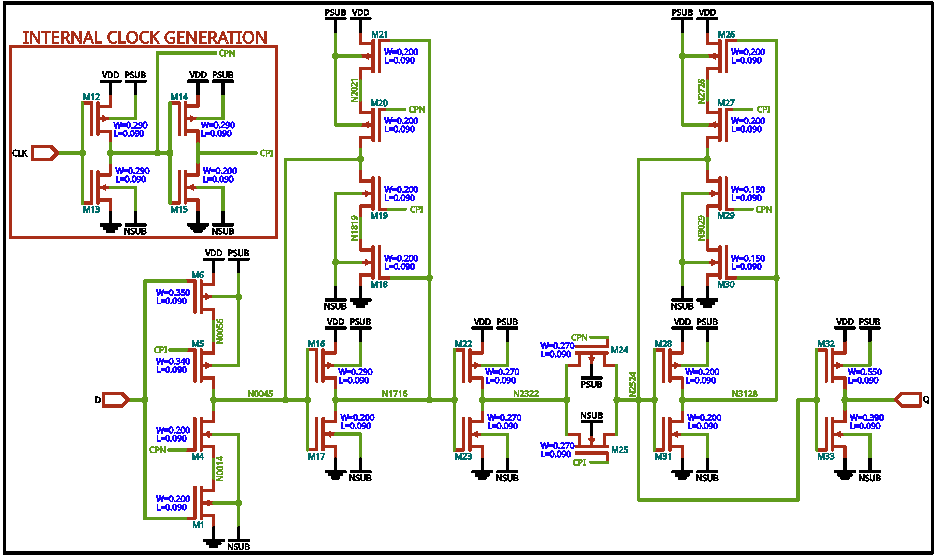
\includegraphics[width=0.5\textwidth]{./figures/CORE65GPSVT_HS65_GS_DFPQX4.pdf}
	\caption{DFF MOS SCH \textcolor{red}{A-T-ON LE DROIT DE METTRE CE SCHÉMA ?}}
\end{figure}

%%	The complete DFF schematic is shown in Fig. \ref{dffmos}.
%
%	Each logic element is connected to four external signals:
%%	The significant extracted signals are the following:
%	\begin{itemize}
%		\item VDD: the power supply voltage;
%		\item VSS: the power supply reference voltage;
%		\item PSUB: the bulk voltage of the PMOS transistors;
%		\item NSUB: the bulk voltage of the NMOS transistors.
%	\end{itemize}
%	These are the signals which are extracted from the SCS simulations.
%	The voltages PSUB and NSUB depend on the substrate type.
%	On the one hand, in the dual-well scenario, NSUB is connected to the epitaxial layer, while PSUB is connected to the N-well.
%	On the other hand, in the triple-well scenario, NSUB is connected to the P-well and PSUB to the N-well.
%	% !TeX spellcheck = en_US
% !TeX root = ./0_article.tex

\begin{figure}[h]
	\label{dffChain}
	\centering
	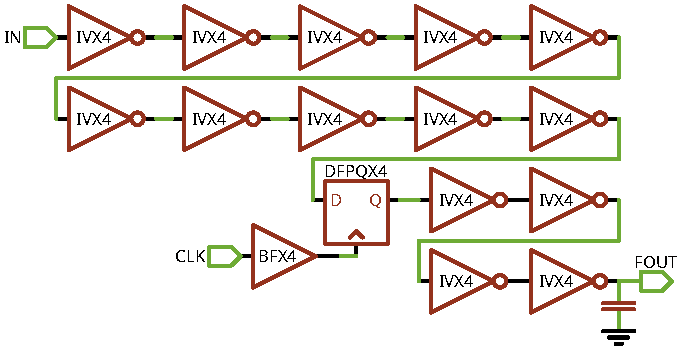
\includegraphics[width=0.5\textwidth]{./figures/dff_ivx_chain_2.pdf}
	\caption{DFFCHAIN}
\end{figure}

%	The resulting simulated logic circuit, combining several inverters, a buffer and a DFF, is shown in Fig. \ref{dffChain}.
%	The first ten inverters, the buffer and the DFF are disturbed thanks to the extracted signals.
%	The four last inverter are not disturbed and are powered with ideal power signals.
%	Their role is to mimic a distant logic block receiving the DFF "BBI disturbed" logic signals.
%	The simulations are performed, as previously, for both a dual-well scenario and a triple-well scenario.
%	However, and for simplicity showing the results, we did not consider the positive pulse case, as we observed high level of destructiveness on actual ICs.
%
%	Presenting such results on a logic path embedding a DFF on a digital or physical static medium is not an easy task.
%	Therefore, we have chosen some specific time during the simulation where we think the results are noteworthy.
%	However, every simulation step is useful to some extent.
%	Therefore, we provide additional simulation results in our GitHub repository dedicated to this paper (\textcolor{red}{mettre repo ?}).
